\subsection{Ejecución en entornos de desarrollo}
\subsubsection{Eclipse}

Para ejecutar la aplicación en un entorno de ejecución como para este caso Eclipse.

\begin{itemize}
	\item Primero se abrirá el entorno de trabajo en la carpeta donde está instalada la aplicación.

	\begin{figure}[H]
		\begin{center}
			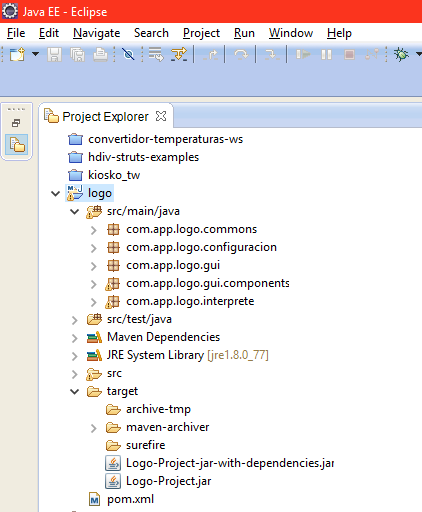
\includegraphics[scale=.4]{images/ejecucion_entorno/eclipse/img_eclipse_0}
			\caption{Menú de selección para ejecutar el proyecto.}
		\end{center}
	\end{figure}
	
	\item Hacer click derecho del icono del proyecto en el panel de 'Proyectos'.
	
	\begin{figure}[H]
		\begin{center}
			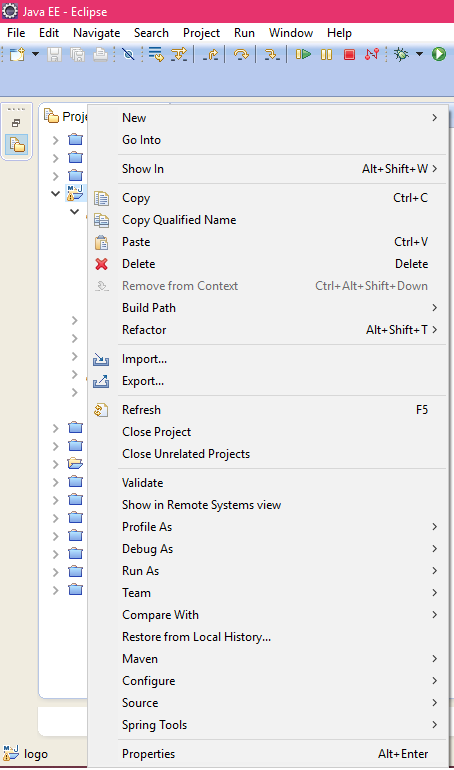
\includegraphics[scale=.4]{images/ejecucion_entorno/eclipse/img_eclipse_1}
			\caption{Menú de selección para ejecutar el proyecto.}
		\end{center}
	\end{figure}	
	
	\item Seleccionar la opción: \textit{Run As}; Finalmente, seleccionar la opción \textit{Maven Install}
	
	\begin{figure}[H]
		\begin{center}
			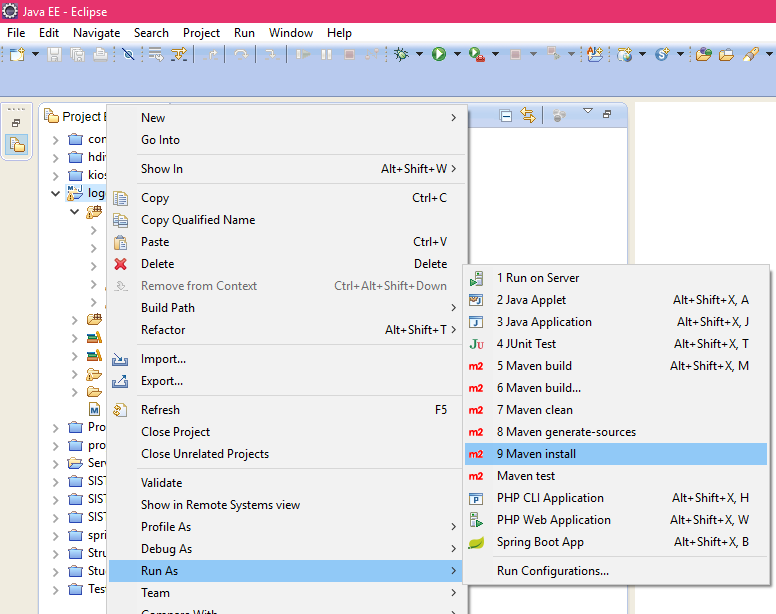
\includegraphics[scale=.4]{images/ejecucion_entorno/eclipse/img_eclipse_2}
			\caption{Ejecutar opción \textit{Maven Install}.}
		\end{center}
	\end{figure}
	
	\item A continuación, se observa la generación de archivos JAR compilados del proyecto.
	
	\begin{figure}[H]
		\begin{center}
			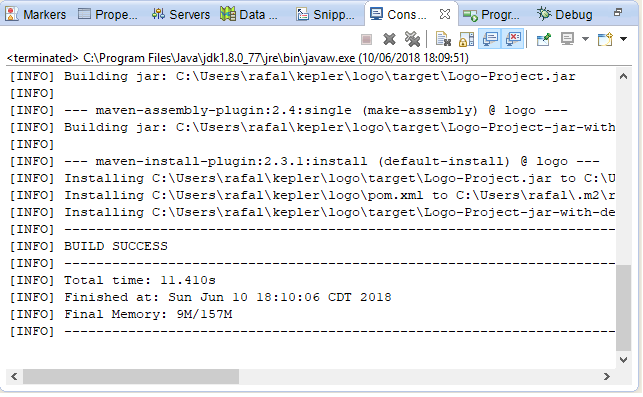
\includegraphics[scale=.4]{images/ejecucion_entorno/eclipse/img_eclipse_3}
			\caption{Generación del proyecto exitosa.}
		\end{center}
	\end{figure}
	
	\begin{figure}[H]
		\begin{center}
			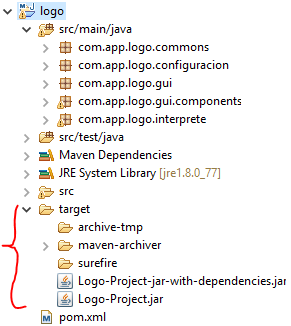
\includegraphics[scale=.4]{images/ejecucion_entorno/eclipse/img_eclipse_4}
			\caption{Carpeta target contiene archivos ejecutables.}
		\end{center}
	\end{figure}
	
\end{itemize}

\subsubsection{Ejecución via terminal}
Para ejecutar la aplicación desde una terminal o CMD, debemos realizar los siguientes pasos:

\begin{itemize}
	\item Dirigirse a la carpeta donde está instalado el archivo <JAR>.
	\item Ejecutar el comando: \textit{java -jar <nombre-archivo>.jar}
\end{itemize}